\documentclass[12pt,a4paper]{article}
\usepackage{graphicx}
\usepackage{caption}
\usepackage{float}
\usepackage[utf8]{inputenc}
\usepackage{amsmath,amssymb,amsthm}
\usepackage{geometry}
\geometry{margin=1in}
\usepackage{hyperref}
\usepackage{listings}
\usepackage{xcolor}

\definecolor{codegray}{rgb}{0.5,0.5,0.5}
\definecolor{codepurple}{rgb}{0.58,0,0.82}
\definecolor{backcolour}{rgb}{0.95,0.95,0.92}

\lstdefinestyle{code}{
    backgroundcolor=\color{backcolour},   
    commentstyle=\color{codegray},
    keywordstyle=\color{blue},
    numberstyle=\tiny\color{codegray},
    stringstyle=\color{codepurple},
    basicstyle=\ttfamily\footnotesize,
    breakatwhitespace=false,         
    breaklines=true,                 
    captionpos=b,                    
    keepspaces=true,                 
    numbers=left,                    
    numbersep=5pt,                  
    showspaces=false,                
    showstringspaces=false,
    showtabs=false,                  
    tabsize=4
}
\lstset{style=code}

\title{Radial Density Functional Theory Solver for Hydrogen-like Atoms}
\author{Jianghai Wang @Nanyang Technological University}
\date{September 2025}

\begin{document}

\maketitle

\section{Introduction}

This repository implements a numerical solution to the Kohn-Sham equations of Density Functional Theory (DFT) for hydrogen-like atoms. The implementation focuses on the radial component of the electronic wavefunction for atoms with spherical symmetry, solving the one-electron case with arbitrary nuclear charge $Z$. This provides a foundational example for understanding self-consistent field (SCF) methods in electronic structure calculations.

\section{Theoretical Background}

\subsection{Density Functional Theory}

Density Functional Theory is a quantum mechanical modeling method used in physics, chemistry, and materials science to investigate the electronic structure of many-body systems. The fundamental principle of DFT is that the properties of a many-electron system can be determined using functionals of the spatially-dependent electron density rather than the many-body wavefunction.

The theoretical foundation of DFT is based on two Hohenberg-Kohn theorems:

\begin{enumerate}
    \item The ground-state properties of a many-electron system are uniquely determined by the electron density.
    \item The electron density that minimizes the energy of the overall functional is the ground-state electron density.
\end{enumerate}

\subsection{Kohn-Sham Equations}

In practice, DFT calculations are performed using the Kohn-Sham approach, which replaces the original many-body problem by an auxiliary independent-particle problem. The Kohn-Sham equation in atomic units is:

\[
\left[-\frac{1}{2}\frac{d^2}{dr^2} + \frac{l(l+1)}{2r^2}+V_\text{KS}(r)\right]P_{nl}(r) = \varepsilon_{nl}P_{nl}(r)
\]

where $P_{nl}(r)=r\Psi_{nl}(r)$ is the radial wave function, and $V_{\text{KS}}(\mathbf{r})$ is the Kohn-Sham potential:

\[
V_{\text{KS}}(\mathbf{r}) = V_\text{nuc}(r) + V_{ee}(r) + V_{xc}(r)
\]

comprising the nuclear attraction potential
\[
V_\text{nuc}(r)=-\frac{Z}{r},
\]
the electron-electron Coulomb repulsion potential
\[
V^{ee}(r) = 4\pi \int \frac{\rho(r')}{|r-r'|} r'^2 dr',
\]
and the exchange-correlation potential $V_{\text{xc}}$.

\subsection{Radial Kohn-Sham Equation}

For atoms with spherical symmetry:
\[
\psi_{nlm}(\mathbf{r}) = \frac{P_{nl}(r)}{r} Y_{lm}(\theta, \phi)
\]

where $Y_{lm}$ are spherical harmonics. For the ground state ($l=0$):
\[
\left[ -\frac{1}{2}\frac{d^2}{dr^2} + V_{{KS}}(r) \right] P_{10}(r) = \varepsilon_{10}P_{10}(r).
\]

\section{Numerical Implementation}

\subsection{Discretization}
\[
r_i = r_0 + i \cdot h, \quad i = 0,1,\dots,N-1
\]

\subsection{Numerov Method}
\[
(1 + \frac{h^2}{12} f_{i+1}) y_{i+1} - (2 - \frac{5h^2}{6} f_i) y_i + (1 + \frac{h^2}{12} f_{i-1}) y_{i-1} = 0,
\]
where $f_i = 2(E - V(r_i))$.

\subsection{Thomas Algorithm}
The Thomas algorithm efficiently solves the tridiagonal system with $O(N)$ complexity.

\subsection{Self-Consistent Field Method}

\begin{figure}[H]
    \centering
    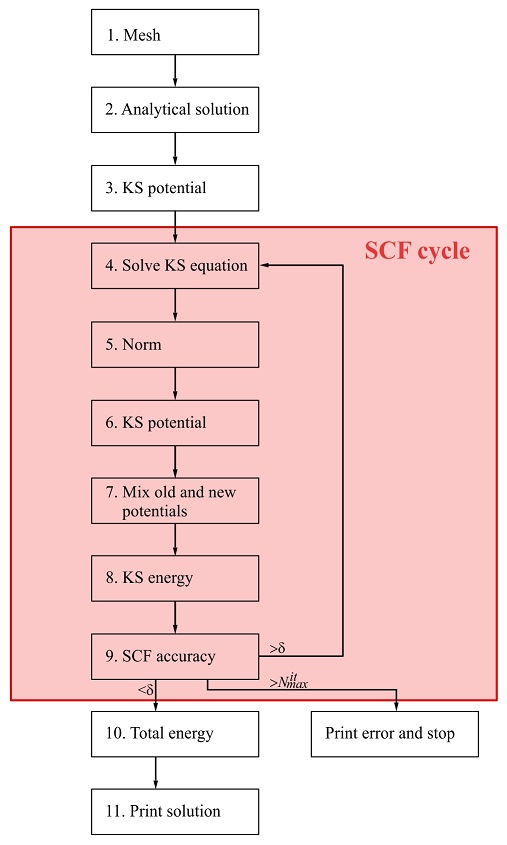
\includegraphics[width=0.7\textwidth]{SCFLoop.jpg}
    \caption{SCF Loop}
\end{figure}

Steps:
\begin{enumerate}
    \item Initialize with an analytical solution
    \item Calculate density
    \item Construct $V_{KS}$
    \item Solve Kohn-Sham equation
    \item Mix potentials
    \item Check convergence
\end{enumerate}

\subsection{Exchange-Correlation Functional}
We implement the Local Density Approximation (LDA).

Exchange:
\[
V^X[\rho] = -\left(\frac{3}{\pi}\rho\right)^{1/3}.
\]

Correlation:
\[
V^C[\rho] =
\begin{cases}
A\ln r_s + \left(B - \tfrac{1}{3}A\right) + \tfrac{2}{3}C r_s \ln r_s + \tfrac{1}{3}(2D-C)r_s, & r_s < 1, \\
\gamma \frac{1 + \tfrac{7}{6}\beta_1 \sqrt{r_s} + \tfrac{4}{3}\beta_2 r_s}{(1 + \beta_1 \sqrt{r_s} + \beta_2 r_s)^2}, & r_s \ge 1.
\end{cases}
\]

where $r_s = \left(\frac{3}{4\pi \rho}\right)^{1/3}$.

\section{Implementation Details}

The \texttt{RadialDFT} class provides:
\begin{itemize}
    \item \texttt{initialize()}, \texttt{normalize()}
    \item \texttt{get\_v\_nuc()}, \texttt{get\_v\_ee()}, \texttt{get\_v\_xc()}
    \item \texttt{solve\_ks()}, \texttt{scf\_loop()}
\end{itemize}

Boundary conditions:
\[
P(r \to 0) \propto r^{l+1}, \quad P(r \to \infty) = 0.
\]

Total energy:
\[
E_{tot} = E_{ks} + E_{ee} + E_{xc} - \int n(r)V_{xc}(r)dr.
\]

\section{Usage}

\subsection{Prerequisites}
Python 3, NumPy, Matplotlib.

\subsection{Running}
Example setup:
\begin{lstlisting}[language=Python]
Z = 6
r0 = 1e-5
rf = 20.0
N = 10001
alpha = 0.1
prec = 1e-5
max_iter = 500
\end{lstlisting}

Run:
\begin{lstlisting}[language=bash]
python main.py
\end{lstlisting}

\subsection{Output}
\begin{enumerate}
    \item \texttt{wavefunction.dat}
    \item \texttt{potential.dat}
    \item \texttt{energy.dat}
    \item \texttt{wavefunction\_comparison.png}
    \item \texttt{potential\_comparison.png}
\end{enumerate}

\section{Validation}

Analytical 1s solution:
\[
P_\text{analytical}(r) = \frac{Z^{3/2}}{\sqrt{\pi}} e^{-Zr}, \quad E = -\frac{Z^2}{2}.
\]

\section{Results and Discussion}

\subsection{Convergence}
Mixing parameter $\alpha$ controls convergence stability.

\subsection{Energy Components}
Final energy breakdown:
\begin{itemize}
    \item Kohn-Sham eigenvalue
    \item Electron-electron repulsion
    \item Exchange-correlation
\end{itemize}

\section{Theoretical Extensions}
Possible improvements:
\begin{enumerate}
    \item Multi-electron systems
    \item GGA/hybrid XC
    \item Excited states
    \item Non-spherical systems
    \item Relativistic effects
\end{enumerate}

\section{Mathematical Appendix}

Radial Schrödinger equation:
\[
\left[-\frac{1}{2r}\frac{d^2}{dr^2}r + \frac{l(l+1)}{2r^2} + V_\text{nuc}(r)\right]\Psi_{nl}(r) = E_{nl}\Psi_{nl}(r).
\]

Numerov recurrence:
\[
\frac{d^2}{d x^2} y(x)+\underbrace{2\left(\varepsilon-V^{K S}(x)\right)}_{f(x)} y(x)=\underbrace{0}_{F(x)}.
\]

Thomas algorithm:
\[
\alpha_{i+1} = -\frac{B_i}{A_i\alpha_i + C_i}, \quad
\beta_{i+1} = \frac{Z_i - A_i\beta_i}{A_i\alpha_i + C_i}.
\]

\section{References}
\begin{enumerate}
    \item Pauling, L.; Wilson, E.B. \textit{Introduction to Quantum Mechanics}, McGraw-Hill, 1935.
    \item Hartree, D.R. \textit{The calculation of atomic structures}. Chapman \& Hall, 1957.
    \item Parr, R.G.; Yang, W. \textit{Density functional theory of atoms and molecules}. Oxford University Press, 1989.
    \item Perdew, J.P.; Zunger, A. Phys. Rev. B 23, 5048 (1981).
    \item Salvadori, M.G. \textit{Numerical methods in engineering}. 1952.
\end{enumerate}

\end{document}